%\linenumbers*

\chapter{IMPLICATION OF IMPROVED CLIGEN ON RAINFALL AND SOIL EROSION
SIMULATIONS}
\label{sec:IMPLICATIONSOFIMPROVEDCLIGEN}

\section{Introduction}
\label{sec:ImprovedCligenIntroduction}
CLIGEN, the weather generator for WEPP, went through extensive modifications
while the current research was carried out \citep{yu2000-301}. The modification
was done to improve CLIGEN in three aspects. The first is the recalculation of
an input parameter, `{MX.5P}', which controls rainfall intensity generations of
CLIGEN. The second is the correction of the unit conversion error in programming
codes of CLIGEN. The third is a subsequent adjustment to shorten the extensive
increases of simulated rainfall durations.

These unforeseen changes prompted an investigation of their implications on
rainfall generations of CLIGEN and, in turn, soil erosion estimations of WEPP.
Before using the improved CLIGEN for this research, it is important to
understand how the improved CLIGEN performs and simulates weather data in
comparison to the previous version.
A first reason for this is to gain insight into CLIGEN's operations. A second
reason is to see how these changes to CLIGEN affect the conclusions made by
previous publications on soil erosion under future climate change. A third
reason is that these changes may have invalidated previous sensitivity analyses
which involved CLIGEN \citep{baffaut1996-447,zhang1996-855,baffaut1998-756,
favis-mortlock1998-141, favis-mortlock1999-329}.

Therefore, this chapter investigates effects of the changes of CLIGEN (from
version 4.2 to version 5.2) on rainfall data simulations and soil erosion
estimations by WEPP. During the investigation process, WEPP is also calibrated
and used for the subsequent simulations of this thesis.

\section{Data Preparation and Method for Model Simulation}
\label{sec:ImprovedCligenMethods}
Firstly, two CLIGEN input files---original and updated (see Appendix
\ref{sec:CLIGENInputData})---were prepared using more recent rainfall data
(Table \ref{tab:DetailsOfDataStations}) obtained from the Ditchling Road site
(Figure \ref{fig:EventRainfallDataSite}). The original CLIGEN input file for
Ditchling Road was used in a study by \citet{favis-mortlock1998-141}. This file
was originally built with help from Arlin Nicks for David Favis-Mortlock in
1992\footnote{From personal communication with David Favis-Mortlock on 3 July
2001: \begin{quotation} ``My problem was that, in 1992, I did not have any
measured intensity data for the area. So, as I recall, I used maps in `NERC
(1975) \textit{Flood Studies Report}, Natural Environment Research Council,
HMSO, London' to pick out the maximum $x$-hour precipitation for each month for
the South Downs, where $x$ is something like 6 hours. The 1975 NERC report was
based on approximately 30 years of data. I then used a chart constructed from
empirical relationships in the 1975 NERC publication---Actually, from data given
to me by someone in the old Southern Water company, which data was drawn from
the 1975 NERC publication---to convert these values into 0.5-hour maxima. I then
sent these 0.5-hour max.\ values to Arlin. From these he calculated time-to-peak
values.'' \end{quotation}}. The newly prepared CLIGEN input file used event data
that have been measured since 1991 (Table \ref{tab:DetailsOfDataStations}).
`MEAN~P' (Table \ref{tab:UpdatedMEANPForDitchlingRoad}) and `{MX.5P}' (Table
\ref{tab:UpdatedMX5PForDitchlingRoad}) values of CLIGEN inputs were recalculated
using the up-to-date event data. Note that the units for these parameters are in
inches, not in millimetres. Only these two parameters were update. The
definition of the `{MX.5P}' was revised by \citet{yu2000-301}, so it was
recalculated accordingly in this research.

\begin{table}[htbp]
  \figureversion{tabular}
  \centering
  \caption[Original and Updated MEAN~P for Ditchling Road]{Original and
Updated MEAN~P (inches) for Ditchling Road}
  \label{tab:UpdatedMEANPForDitchlingRoad}
    \footnotesize
    \begin{tabular}{lrrrrrrrrrrrr}
    \toprule
     & Jan & Feb & Mar & Apr & May & Jun & Jul & Aug & Sep & Oct &
Nov & Dec\\
    \cmidrule{2-13}
    Original & 0.19 & 0.16 & 0.17 & 0.16 & 0.16 & 0.20 & 0.19 & 0.22
& 0.23 & 0.27 & 0.21 & 0.20\\
    Updated & 0.11 & 0.11 & 0.18 & 0.21 & 0.17 & 0.15 & 0.16 & 0.13
& 0.24 & 0.29 & 0.19 & 0.29\\
    \bottomrule
    \end{tabular}
\end{table}

\begin{table}[htbp]
  \figureversion{tabular}
  \centering
  \caption[Original and Updated {MX.5P} for Ditchling Road]{Original and
Updated {MX.5P} (in/hr) for Ditchling Road}
  \label{tab:UpdatedMX5PForDitchlingRoad}
    \footnotesize
    \begin{tabular}{lrrrrrrrrrrrr}
    \toprule
     & Jan & Feb & Mar & Apr & May & Jun & Jul & Aug & Sep & Oct &
Nov & Dec\\
    \cmidrule{2-13}
    Original & 0.63 & 0.59 & 0.55 & 0.55 & 0.55 & 0.55 & 0.55 & 0.67
& 0.79 & 0.93 & 0.87 & 0.75\\
    Updated & 0.27 & 0.18 & 0.23 & 0.23 & 0.27 & 0.33 & 0.42 & 0.58
& 0.43 & 0.45 & 0.34 & 0.30\\
    \bottomrule
    \end{tabular}
\end{table}

Next, continuous daily climate data for 30 years were generated with CLIGEN
version 4.1\footnote{There is virtually no difference between version 4.1 and
4.2 although version 4.2 was the one \citet{yu2000-301} found error in.} (old)
and version 5.2 (new) using these two input files. As a result, four datasets of
simulated climate data were generated (Table
\ref{tab:CLIGENSimulationSettingsWithDifferentInputsAndVersions}). These climate
data were compared in terms of rainfall amount, duration and peak intensity.

\begin{table}[htbp]
  \centering
  \small
  \caption{Weather simulation settings with different CLIGEN versions and inputs
for Ditchling Road}
  \label{tab:CLIGENSimulationSettingsWithDifferentInputsAndVersions}
  \begin{tabular}{ccc}
  \toprule
        & Original Input & Updated Input \\
  \midrule
  CLIGEN v4.1 & v4.1+original & v4.1+updated \\
  \midrule
  CLIGEN v5.2 & v5.2+original & v5.2+updated \\
  \bottomrule
  \end{tabular}
\end{table}

Two combinations of data and CLIGEN (i.e.\ v4.1+original and v5.2+updated) are
of the main concerns in this chapter because the other combinations (i.e.\
v5.2+orginal and v4.1+updated) have ``invalid'' combinations of MEAN~P and
{MX.5P}. Thus, the latter combinations will not give realistic results.
They are only considered here to highlight the changes of CLIGEN as a
sensitivity test.

Using WEPP, soil erosion rates for the same thirty-year period were, in turn,
estimated for Woodingdean site (Figure \ref{fig:WoodingdeanSite}) with each
CLIGEN-generated climate dataset. All other input data for the WEPP simulation
were acquired from the previous study by \citet{favis-mortlock1998-141}. Runoff
and soil loss rates were compared.
Kolmogorov-Smirnov (K-S) test was used to test the null hypothesis that the two
populations are identical. Results of K-S test are presented in the next
section.

\section{Implication on Rainfall Data Simulation}
\label{sec:RainfallSimulation}

\subsection{Rainfall Amount}
Generated annual rainfall amounts for 30 years were within the range of the
reported annual rainfall amounts (750 and 1000 mm) in the area (Figure
\ref{fig:cligen_annual_amount}). The annual rainfall amounts generated by two
input files were not significantly different (K-S test, $p<0.05$). Although two
versions of CLIGEN resulted in a slight difference in annual rainfall amounts in
year 17 (Figure \ref{fig:cligen_annual_amount}), the differences between two
versions of CLIGEN were not statistically significant (K-S test, $p<0.05$).

\begin{figure}[htbp]
  \centering
   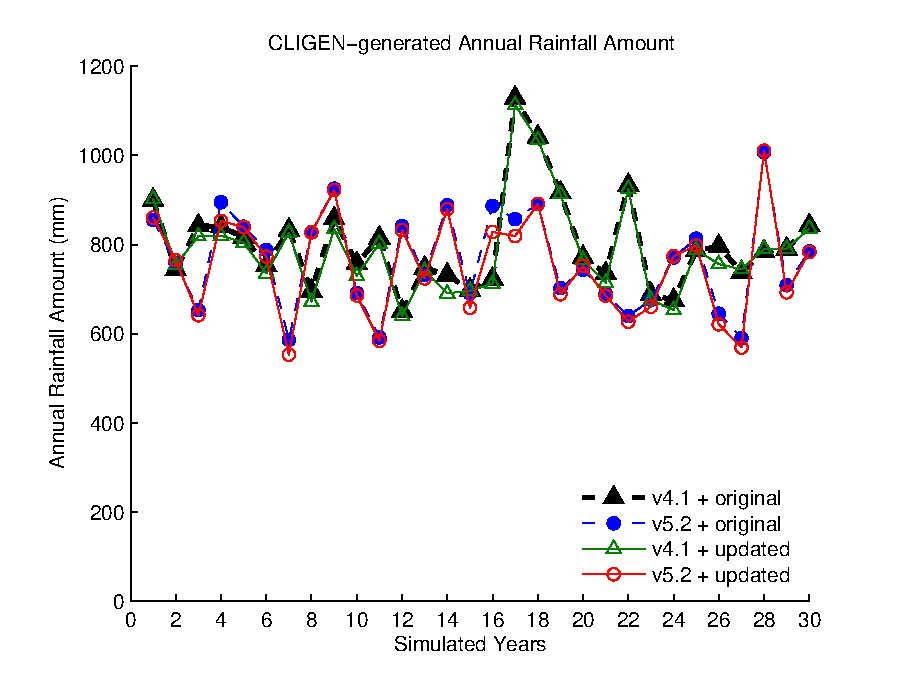
\includegraphics[width=0.8\textwidth]{./img/cligen_annual_amount_series}
  \caption{Simulated annual rainfall amount using two versions of CLIGEN with
original and updated input files.}
  \label{fig:cligen_annual_amount}
\end{figure}

\subsection{Rainfall Duration}
Contrastingly, simulated annual rainfall durations using two versions of CLIGEN
exhibited noticeable differences. Old version of CLIGEN generated identical
annual rainfall durations even though two different input files (original
and updated) were used (Figure \ref{fig:cligen_annual_duration}). New CLIGEN
generated markedly different rainfall durations when the same set of CLIGEN
input files were used (Figure \ref{fig:cligen_annual_duration}) (K-S test,
$p<0.05$).

\begin{figure}[htbp]
  \centering
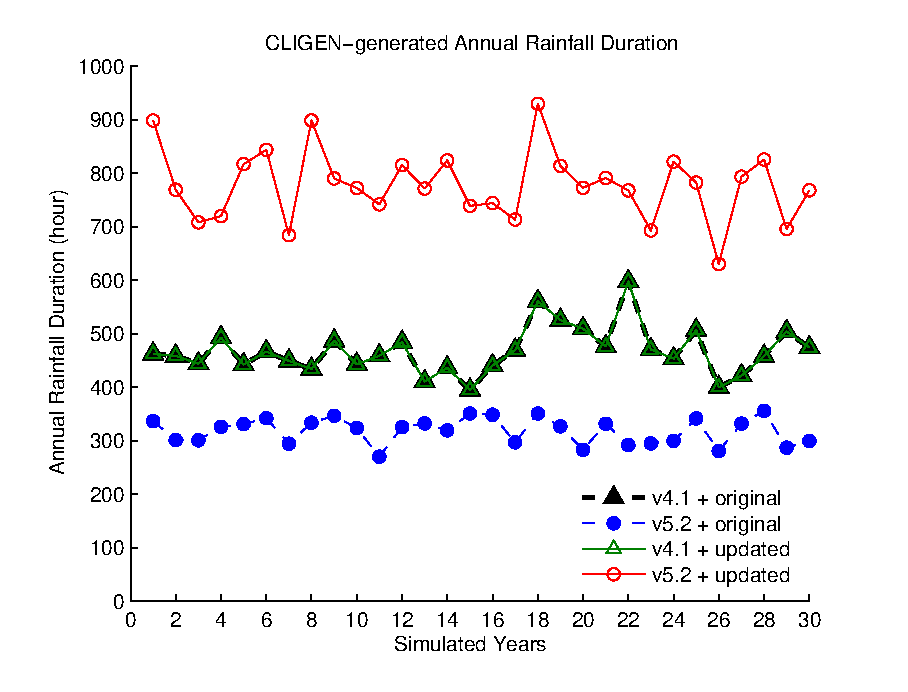
\includegraphics[width=0.8\textwidth]{./img/cligen_annual_duration_series}
  \caption{Simulated annual rainfall duration using two versions of CLIGEN
with original and updated input files.}
  \label{fig:cligen_annual_duration}
\end{figure}

New CLIGEN with updated input file generated greatly increased rainfall
durations, almost 2.5 times longer on average than with original input file. The
rainfall duration (v5.2 + updated) was over 1.5 times longer on
average in comparison to the rainfall duration generated by old CLIGEN with both
original and updated input files. New CLIGEN with original input file
generated the shortest annual rainfall durations among the four series.
This means that, unlike old version, new version of CLIGEN is sensitive to
the change of two CLIGEN input parameters (i.e.\ MEAN~P and {MX.5P}),
particularly to the change of {MX.5P}. These large differences in rainfall
durations mean that rainfall intensities also differ greatly between the
simulated rainfall datasets.

\subsection{Monthly Maxima of Daily Peak Rainfall Intensity}
Next, monthly maxima of daily peak rainfall intensity series generated by CLIGEN
were compared in order to examine effects of extreme intensity events. The
results are shown in Figure \ref{fig:cligen_monthly_max_int}.
Kolmogorov-Smirnov test indicates that old CLIGEN was not sensitive to the
changes of input files (See Figure \ref{fig:cligen_monthly_max_int}(a) and
\ref{fig:cligen_monthly_max_int}(c), $p<0.05$). In contrast, using original and
updated input files with new CLIGEN resulted in two significantly (K-S test,
$p<0.05$) different distributions of monthly maxima of daily peak rainfall
intensity (See Figure \ref{fig:cligen_monthly_max_int}(b) and
\ref{fig:cligen_monthly_max_int}(d)).
New CLIGEN generated fewer high intensity events than the old version (Figure
\ref{fig:cligen_monthly_max_int}(a)(c) and
\ref{fig:cligen_monthly_max_int}(b)(d)). There were, for example, only nine
monthly maxima of daily peak intensity over 100 mm/hr during 30 years of the
simulation period when new CLIGEN and updated input file were used (Figure
\ref{fig:cligen_monthly_max_int}(d)). The magnitude of the monthly maxima of the
daily peak intensity seems to be in a similar range for all four cases although
the frequency of the high peaks are different depending on the version of
CLIGEN and input files (Figure \ref{fig:cligen_monthly_max_int}).

\begin{figure}[htbp]
  \centering

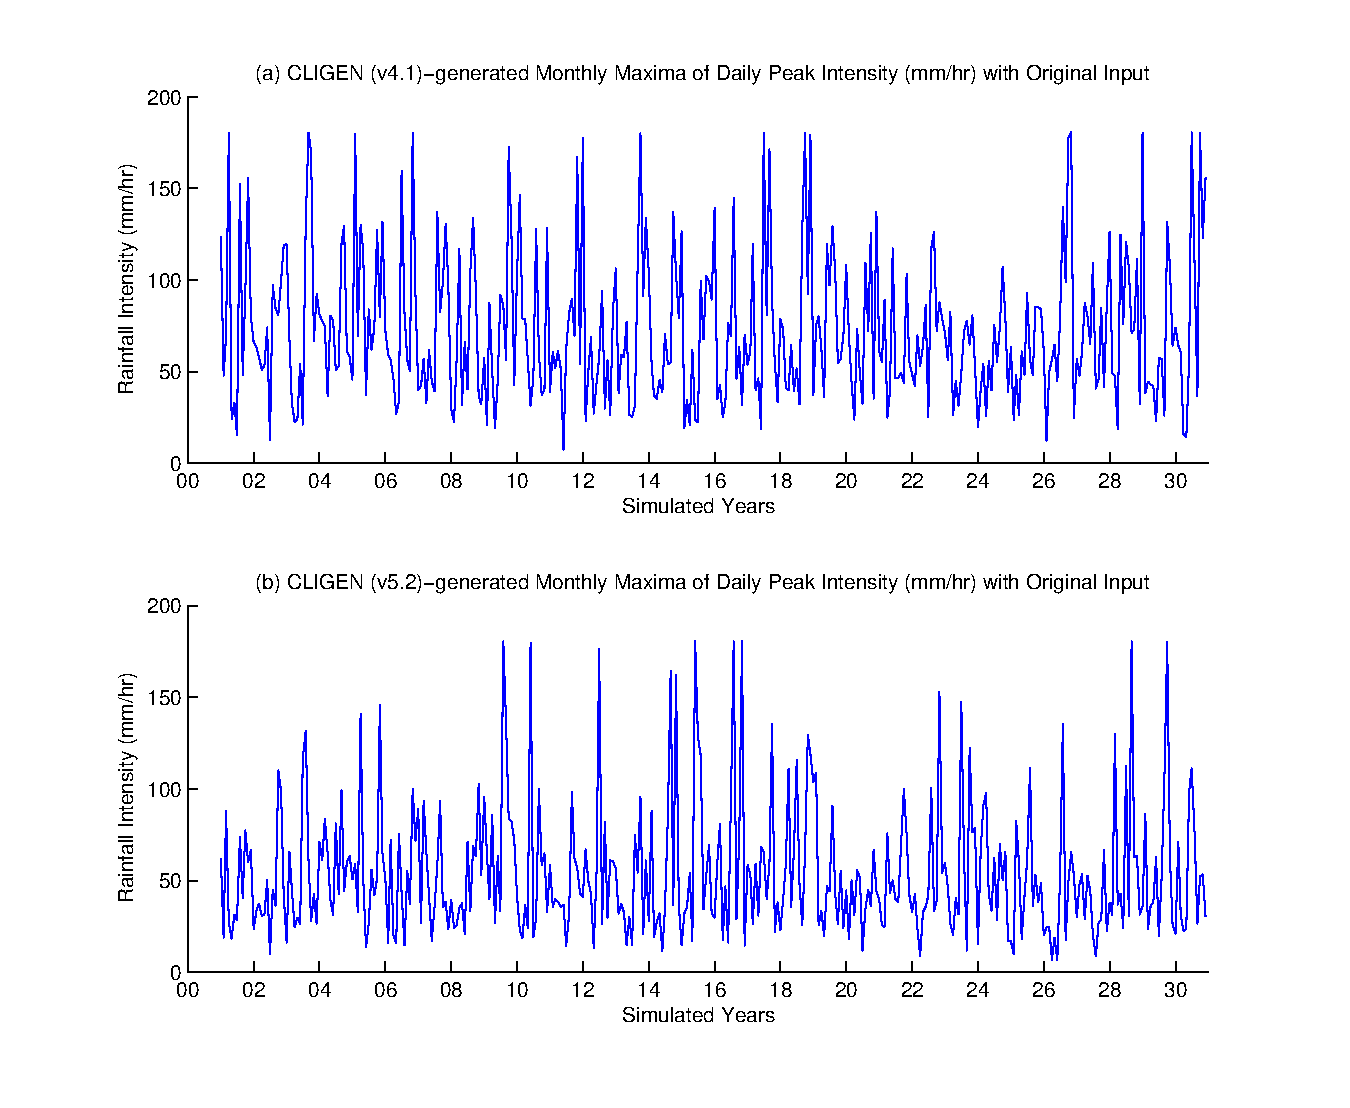
\includegraphics[width=0.8\textwidth]{./img/cligen_monthly_max_int_org}

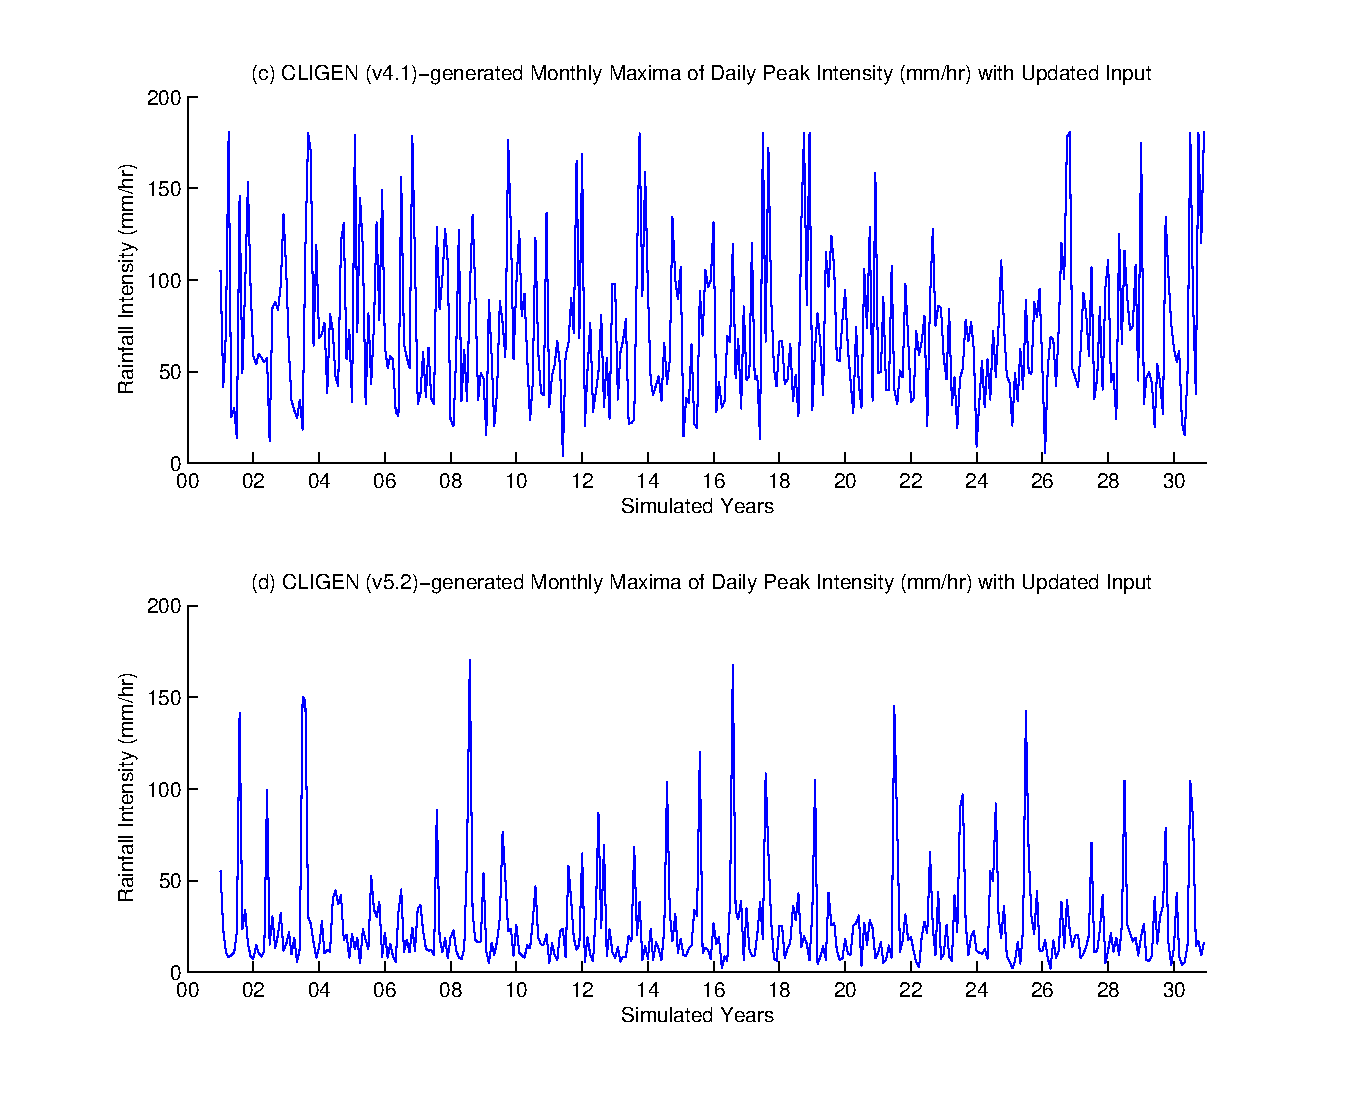
\includegraphics[width=0.8\textwidth]{./img/cligen_monthly_max_int_mod}
  \caption[Simulated monthly maxima of daily peak rainfall intensity using
two versions of CLIGEN with original and updated input files]{Simulated monthly
maxima of daily peak rainfall intensity using two versions of CLIGEN with
original and updated input files. (a) CLIGEN v4.1 with original input file; (b)
CLIGEN v5.2 with original input file; (c) CLIGEN v4.1 with updated input file;
(d) CLIGEN v5.2 with updated input file.}
  \label{fig:cligen_monthly_max_int}
\end{figure}

\begin{figure}[htbp]
  \centering
    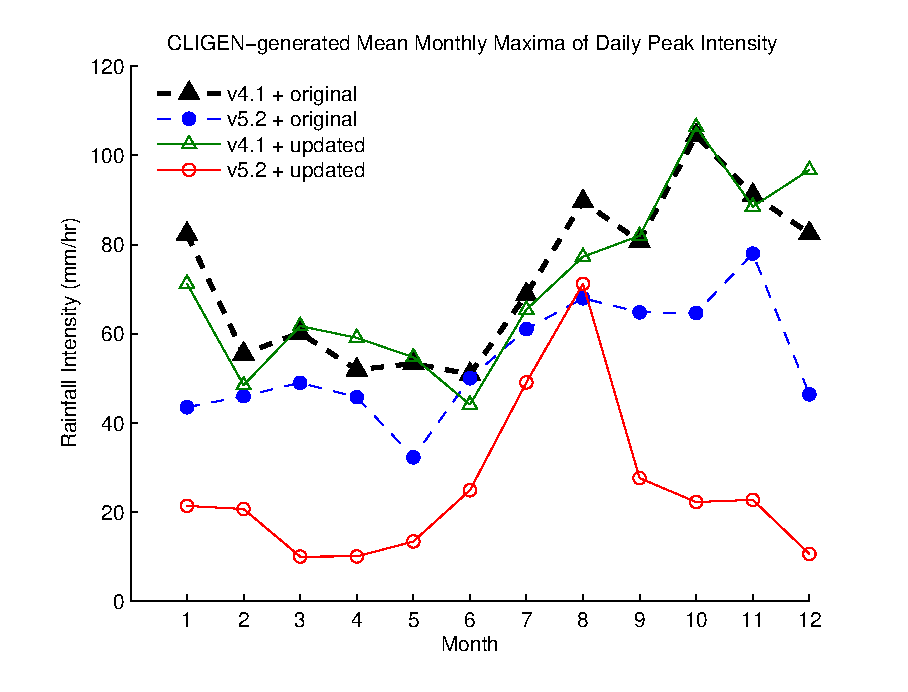
\includegraphics[width=0.8\textwidth]{./img/cligen_monthly_max_int_by_month}
  \caption{CLIGEN-generated mean monthly maxima of daily peak intensity
using two versions of CLIGEN with original and updated input files}
  \label{fig:cligen_dr_monthly_max_int_by_month}
\end{figure}

Mean monthly maxima of daily peak intensity were compared in Figure
\ref{fig:cligen_dr_monthly_max_int_by_month}. Old CLIGEN with two input files
generated generally high mean monthly values through out most of months in
comparison to new CLIGEN. The effect of different input files was very small
on old CLIGEN for simulating mean monthly maxima of daily peak intensity. Old
CLIGEN generated highest mean monthly maxima of daily peak intensity in October
and lowest values in June with both input files. In contrast, new CLIGEN
generated significantly different mean monthly maxima of daily peak intensity
with two input files (K-S test, $p<0.05$). Much greater mean monthly maxima of
daily peak intensity were generated with v5.2 + original than with v5.2 +
updated. With original input file, new CLIGEN (v5.2) showed a peak in
November and a low in May.

With exception of v5.2 + updated, all three simulations show generally high mean
monthly maxima of daily peak intensity in October and November and low mean
monthly maxima of daily peak intensity in April, May and June. When new CLIGEN
with updated input file were used for the simulation, the monthly pattern was
very different from that of the other three combinations. In other words,
nev CLIGEN with updated input file (v5.2 + updated) simulated more realistic
monthly rainfall intensity.
This combination (i.e.\ v5.2 + updated) showed relatively high mean monthly
maxima of daily peak intensity during the summer months (June, July and August)
with a distinctively high peak in August (Figure
\ref{fig:cligen_dr_monthly_max_int_by_month}). Generally low mean monthly maxima
of daily peak intensity in the rest of months were simulated with lowest mean
monthly maxima of daily peak intensity in March and April (Figure
\ref{fig:cligen_dr_monthly_max_int_by_month}). With updated input file and new
CLIGEN, more high intensity events were simulated in the summer than the autumn
or winter in comparison to the other simulation combinations. This result is
closely similar to observed rainfall intensity found previously (Figure
\ref{fig:obs_mean_monthly_30min_intensity})
%reason for this result can be explained by looking at the input files, october
%and august, MEAN P and MX .5P

\section{Implication on Runoff and Soil Erosion Simulation}
\label{sec:RunoffAndSoilLossSimulation}
Before starting investigations on effects of improved CLIGEN on WEPP
simulations, initial tests of WEPP were carried out with weather generated by
new CLIGEN with updated input file. The tests revealed that uncalibrated WEPP
overestimates mean soil loss by about 630\% in comparison to observed soil
losses from the study area (Table
\ref{tab:SimulatedSoilLossWithCLIGENV52WithUpdatedInput}). This erosion rate is
considered unrealistically high for the study site so that calibrations is
considered essential.

\begin{table}[htbp]
  \figureversion{tabular}
  \centering
  \caption[Simulated annual average runoff on hillslopes using
CLIGEN-generated weather with updated input]{Simulated annual average runoff
(mm) on hillslopes (D-L) using CLIGEN-generated (v5.2) weather with updated
input}
  \label{tab:SimulatedRunoffWithCLIGENV52WithUpdatedInput}
  \small
    \begin{tabular}{lrrrrrrrrrr}
      \toprule
      & D & E & F & G & H & I & J & K & L & Mean\\
      \cmidrule{2-11}
      uncalib. & 106.7 & 105.3 & 106.5 & 106.0 & 106.1 & 107.1
& 107.8 & 108.0 & 108.8 & 106.9\\
      recalib. & 74.2 & 72.9 & 73.9 & 73.6 & 73.4 & 74.3 &
74.8 & 75.2 & 75.9 & 74.2\\
      \bottomrule
    \end{tabular}
\end{table}

\begin{table}[htbp]
  \figureversion{tabular}
  \centering
  \caption[Simulated annual average soil loss on hillslopes using
CLIGEN-generated weather with updated input]{Simulated annual average soil loss
(t/ha) on hillslopes (D-L) using CLIGEN-generated (v5.2) weather with updated
input}
  \label{tab:SimulatedSoilLossWithCLIGENV52WithUpdatedInput}
  \footnotesize
    \begin{tabular}{lrrrrrrrrrr}
      \toprule
      & D & E & F & G & H & I & J & K & L & Mean\\
      \cmidrule{2-11}
      uncalibrated & 49.4 & 42.9 & 76.1 & 96.5 & 117.5 & 111.1
& 105.3 & 84.1 & 79.7 & 84.7\\
      recalibrated & 3.4 & 3.2 & 11.1 & 18.2 & 23.7 & 21.3 &
17.3 & 9.8 & 7.9 & 12.8\\
      measured$^a$ (m$^3$/ha) & 3.4 & 7.8 & 13.7 & 17.5 & 21.4
& 9.6 & 11.6 & 11.2 & 8.1 & 11.6\\
      \bottomrule
      %\addlinespace[1mm]
      \multicolumn{8}{l}{\footnotesize $^a$ over the periods
of 1985-1986 \citep[From][]{favis-mortlock1998-141}}
    \end{tabular}
\end{table}

Thus, WEPP was calibrated by adjusting hydrological and
erosional parameter values. The adjusted parameters were shown in Table
\ref{tab:HydrologicalAndErosionalParameters}. Simulated runoff and soil
loss rates using uncalibrated and calibrated WEPP are presented in Table
\ref{tab:SimulatedRunoffWithCLIGENV52WithUpdatedInput} and
\ref{tab:SimulatedSoilLossWithCLIGENV52WithUpdatedInput}. There were no measured
runoff data available for the site although annual soil loss data for a short
period were acquired from \citet{favis-mortlock1998-141}.

\paragraph{Why Calibrate?} It is paramount to test and calibrate a model before
using it in the subsequent investigation of this research. When a erosion model
is used for soil loss estimations, it is important to note that the relationship
of model inputs and outputs is non-linear
\citep{favis-mortlock1995-365,jetten1999-521}. For example, say, we ran a
erosion model with \emph{Input A} and got \emph{Output B}
(Figure \ref{fig:calibration}).

\begin{figure}[htbp]
  \centering
    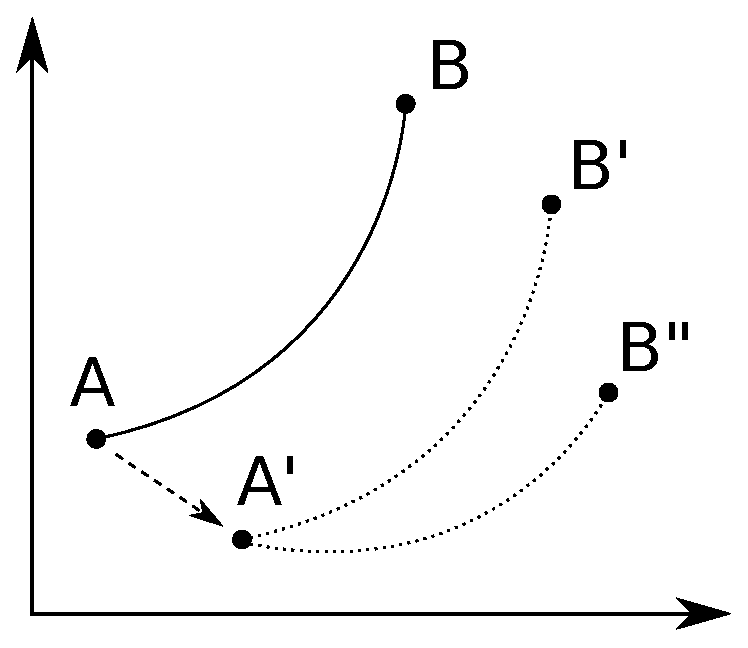
\includegraphics[width=0.5\textwidth]{./img/calibration}
  \caption{A graphical representation of non-linear responses of a erosion
model}
  \label{fig:calibration}
\end{figure}

Then, in order to find possible effects of changes in inputs, we may change
\emph{Input A} to \emph{Input A'}. When the model was run with \emph{Input A'},
the responding model output should be \emph{Output B'} if the model has a linear
relationship between inputs and outputs. However, because of the non-linear
relationship, the responding output may be rather unknown \emph{Output B''}
(Figure \ref{fig:calibration}). This means that, unless model inputs and outputs
are identified and the model is calibrated against known output values, it may
be difficult to measure the extent of changes in model predictions.

Therefore, it is very unlikely that non-calibrated models will lead to
reasonable simulation results. However, even after calibration, there still is
the possibility of ending up with `the right answer for the wrong reason'
\citep{favis-mortlock1994-use}. This is, for example, because two or more model
inputs cancel each other out (or enhance each other) by unknown interactions.

WEPP simulated annual runoff and soil loss rates using four CLIGEN-generated
weather series are shown in Figure \ref{fig:cligen_annual_runoff_serise} and
Figure \ref{fig:cligen_annual_sloss_series}, respectively.

\begin{figure}[htbp]
  \centering
    \subfloat[]{%
    \label{fig:cligen_annual_runoff_serise_a}
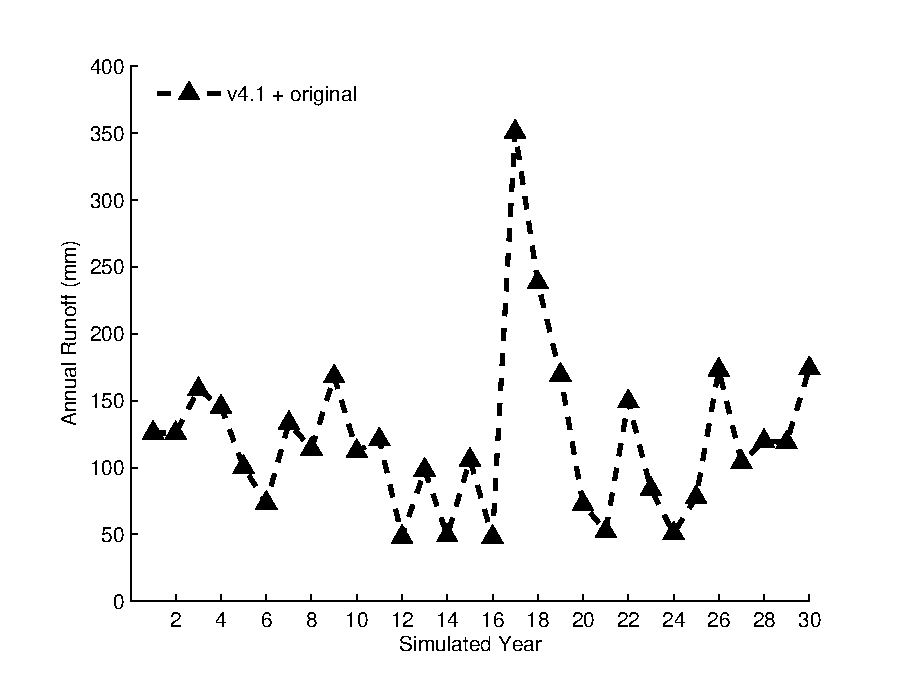
\includegraphics[width=0.49\textwidth]
{./img/cligen_annual_runoff_serise_old_original}}
    \subfloat[]{%
    \label{fig:cligen_annual_runoff_serise_b}
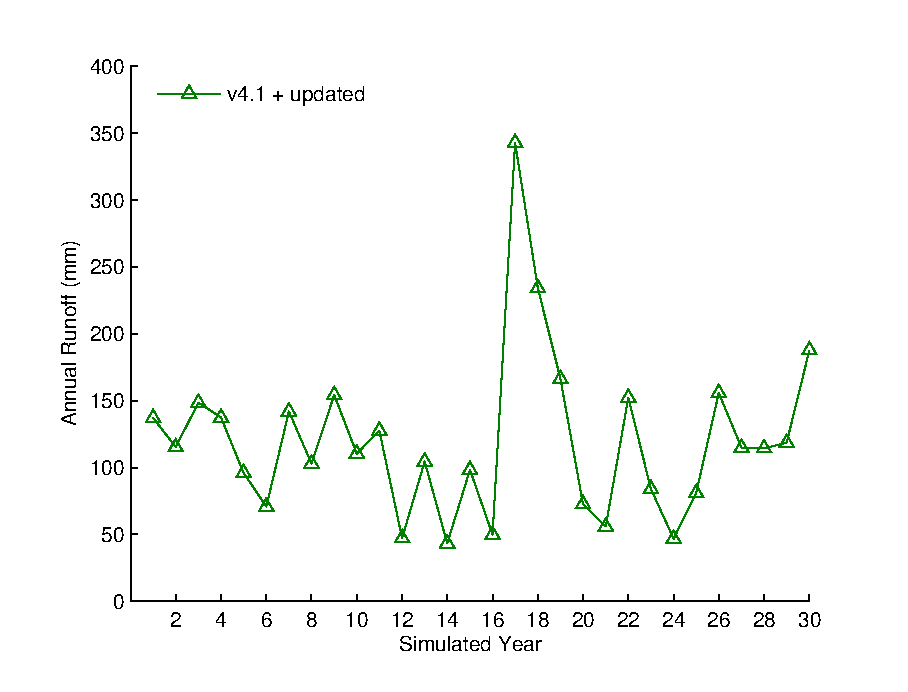
\includegraphics[width=0.49\textwidth]{%
./img/cligen_annual_runoff_serise_old_updated}}
    \qquad
    \subfloat[]{%
    \label{fig:cligen_annual_runoff_serise_c}
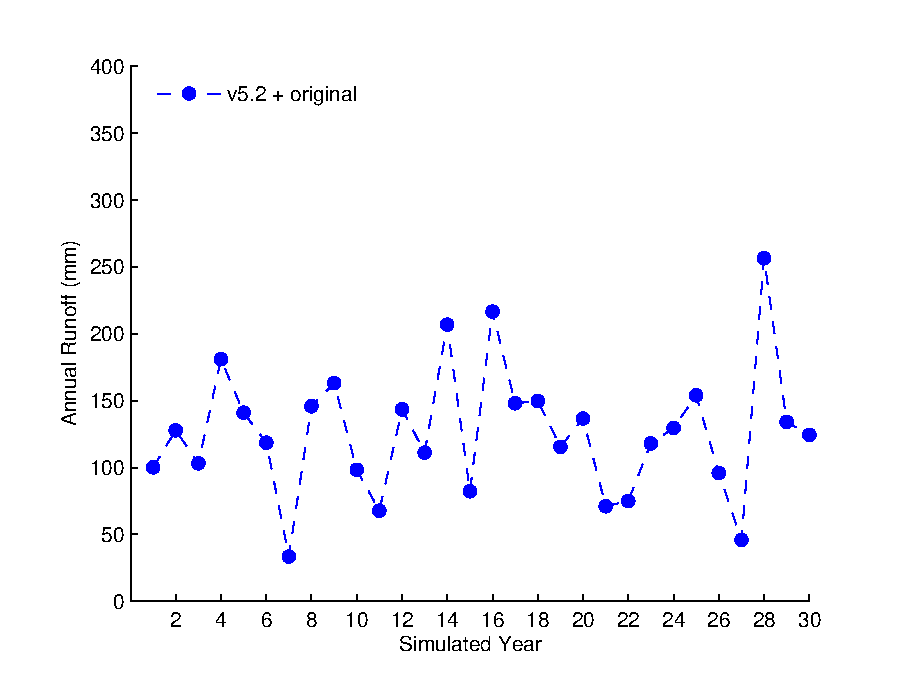
\includegraphics[width=0.49\textwidth]{%
./img/cligen_annual_runoff_serise_new_original}}
    \subfloat[]{%
    \label{fig:cligen_annual_runoff_serise_d}
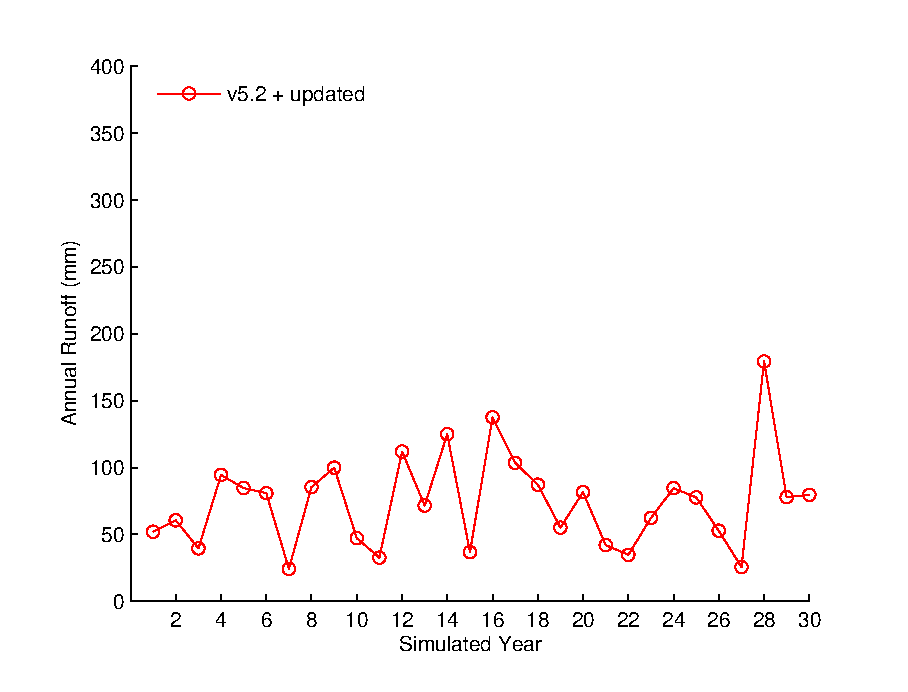
\includegraphics[width=0.49\textwidth]{%
./img/cligen_annual_runoff_serise_new_updated}}
  \caption[Simulated annual runoff for Ditchling Road]{Simulated annual
runoff for Ditchling Road simulated with (a) old CLIGEN with original input
file; (b) old CLIGEN with updated input file; (c) new CLIGEN with original input
file; (d) new CLIGEN with updated input file. Note the same Y-axis in plots.}
  \label{fig:cligen_annual_runoff_serise}
\end{figure}

\begin{figure}[htbp]
  \centering
  \subfloat[]{%
  \label{fig:cligen_annual_sloss_series_a}
  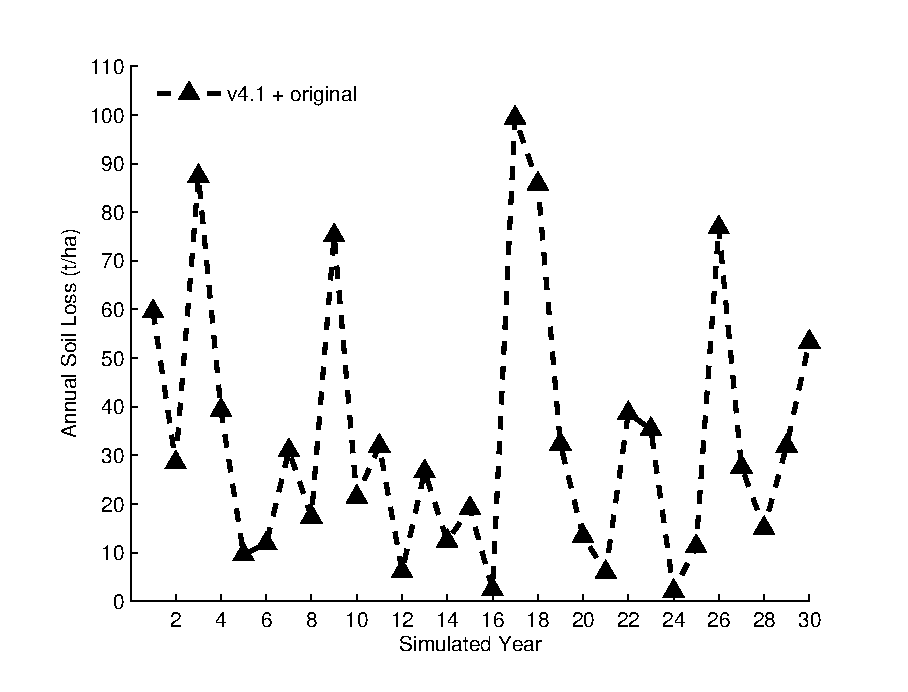
\includegraphics[width=0.49\textwidth]{%
./img/cligen_annual_sloss_serise_old_original}}
  \subfloat[]{%
  \label{fig:cligen_annual_sloss_series_b}
  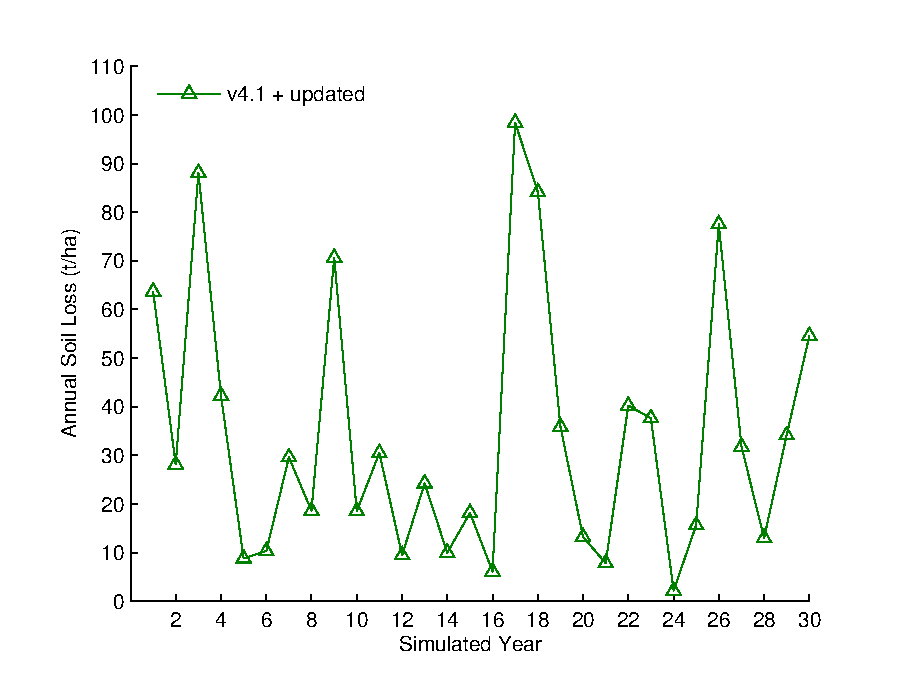
\includegraphics[width=0.49\textwidth]{%
./img/cligen_annual_sloss_serise_old_updated}}
  \qquad
  \subfloat[]{%
  \label{fig:cligen_annual_sloss_series_c}
  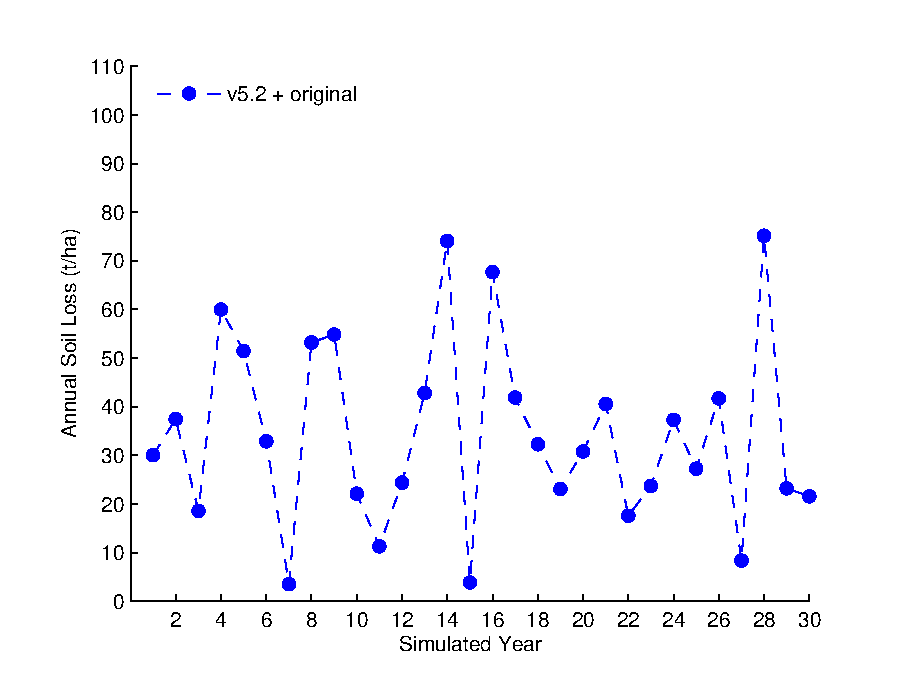
\includegraphics[width=0.49\textwidth]{%
./img/cligen_annual_sloss_serise_new_original}}
  \subfloat[]{%
  \label{fig:cligen_annual_sloss_series_d}
  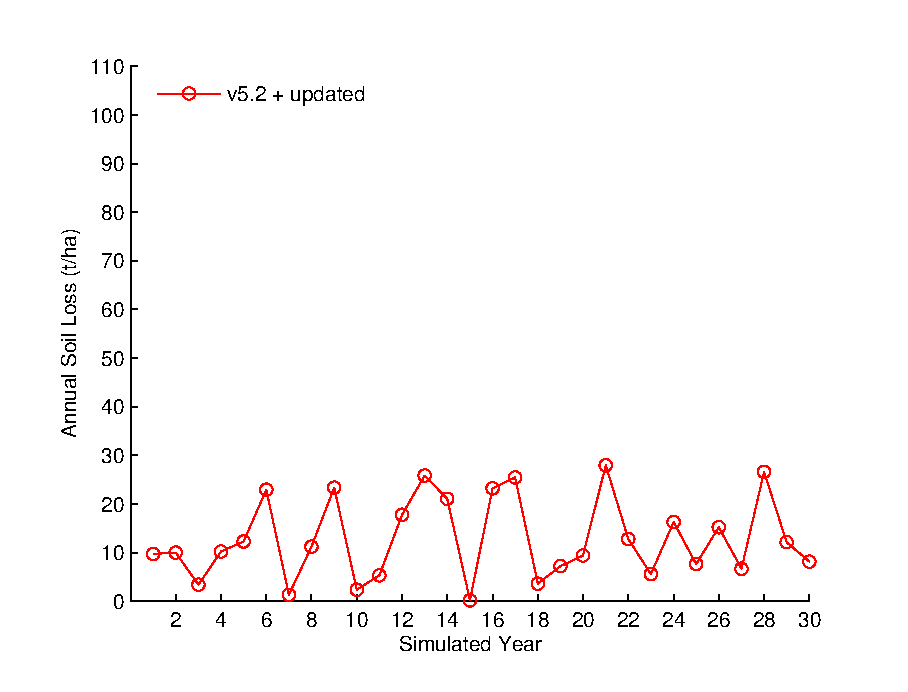
\includegraphics[width=0.49\textwidth]{%
./img/cligen_annual_sloss_serise_new_updated}}
  \caption[Simulated annual soil loss for Ditchling Road]{Simulated annual
soil loss for Ditchling Road simulated with (a) old CLIGEN with original input
file; (b) old CLIGEN with updated input file; (c) new CLIGEN with original input
file; (d) new CLIGEN with updated input file. Note the same Y-axis in plots.}
  \label{fig:cligen_annual_sloss_series}
\end{figure}

Annual runoff and soil loss rates were not significantly affected by the use of
weather datasets that have been generated by old CLIGEN (v4.1) with two input
files (original and updated). Annual runoff (Figure
\ref{fig:cligen_annual_runoff_serise_a} and Figure
\ref{fig:cligen_annual_runoff_serise_b}) and annual soil loss rates (Figure
\ref{fig:cligen_annual_sloss_series_a} and Figure
\ref{fig:cligen_annual_sloss_series_b}) were almost identical between the two
configurations (v4.1 + original and v4.1 + updated). However, this is reasonable
given that there is little difference in the rainfall amounts and peak rainfall
intensities for these combinations (Figure \ref{fig:cligen_monthly_max_int}).

Mean annual runoff and soil
loss rates estimated using weather data generated by v4.1 + updated were
slightly decreased by 1.4\% and increased by 1.5\% respectively in comparison to
the estimation done by the use of weather data generated with v4.1 + original
(Table \ref{tab:SimualtedAnnualRunoffAndSoilLossWithDifferentConfiguration}).

\begin{table}[htbp]
  \figureversion{tabular}
  \centering
  \caption[WEPP simulated average annual runoff and soil loss]{WEPP
simulated average annual runoff (mm) and soil loss (t/ha) with CLIGEN generated
weather with four different configurations.}
  \label{tab:SimualtedAnnualRunoffAndSoilLossWithDifferentConfiguration}
    \begin{tabular}{lrrrr}
      \toprule
       & \multicolumn{2}{c}{CLIGEN v4.1} &
\multicolumn{2}{c}{CLIGEN v5.2}\\
      \cmidrule(r){2-3}\cmidrule(l){4-5}
       & original input & updated input & original input &
updated input \\
      \midrule
      Runoff & 122.1 & 120.4 ($-$1.4) & 126.5 ($+$3.6) & 74.2 ($-$39.2)\\
      Soil Loss & 33.6 & 34.1 ($+$1.5) & 34.4 ($+$2.4) & 12.8 ($-$61.9)\\
      \bottomrule
      %\addlinespace[1mm]
      \multicolumn{5}{p{10.5cm}}{\footnotesize Figures in (\ )
represent \% differences from CLIGEN v4.1+original input file. $+/-$ sign
indicates an increase/decrease.}
    \end{tabular}
\end{table}

When both CLIGENs (v4.1 and v5.2) were run with original input file to generate
weather data, subsequent WEPP estimations of average annual runoff and soil loss
were not much different between the two versions of CLIGEN. Average annual
runoff and soil loss were only increased by 3.6\% and 2.4\%, respectively.
(Table \ref{tab:SimualtedAnnualRunoffAndSoilLossWithDifferentConfiguration}).

WEPP estimated considerably decreased runoff and soil loss rates when rainfall
data generated by new CLIGEN with updated input file were used (Figure
\ref{fig:cligen_annual_runoff_serise_d} and Figure
\ref{fig:cligen_annual_sloss_series_d}) in comparison to the other three
configurations (Figures
\ref{fig:cligen_annual_runoff_serise_a}--c and Figures
\ref{fig:cligen_annual_sloss_series_a}--c). This result is consistent with the
result from rainfall simulations. In comparison to mean runoff and soil loss
rates estimated using rainfall data generated by old CLIGEN with
original input file, the runoff and soil loss rates decreased by about 39\% and
about 62\% respectively when rainfall data generated by new CLIGEN with updated
input file were used for WEPP simulations (Table
\ref{tab:SimualtedAnnualRunoffAndSoilLossWithDifferentConfiguration}).
The importance of these results are discussed in the following section.

\paragraph{Relative vs Absolute Model Output} In this research, both relative
(\% change) and absolute (t/ha) values were used for model outputs. It may seem
more meaningful to use only relative representations (\% change) of model
outputs than to use absolute values (t/ha) together with \% changes because what
this research is interested in is how model estimates change as a result of
rainfall intensity changes. However, in order to make a right judgement and to
assess estimated values correctly, we need both expressions: relative and
absolute. For instance, if a model estimates soil loss of 1000 t/ha from
a 1 m$\times$1 m plot after 10 mm/hr rainfall, it would hardly be considered
realistic, and the model and its inputs may need to be checked to find a reason
for the error. On the other hand, when a model estimates soil loss that changes
from, say, 0.00001 t/ha to 0.00002 t/ha, the \% change would be 100\% despite
the fact that this value can be seen as very trivial in the real world. Thus,
presenting the model result either only in relative (\% change) or absolute
(t/ha) value is probably misleading. Therefore, both expressions are used in
this research when simulation results are presented.
%Also, calibrations carried
%out previously provide robust realistic absolute values.

\section{Discussion}
\label{sec:ImprovedCLIGENDiscussion}

\subsection{Impact on Rainfall Intensity Generation}

\citet{yu2000-301} suggests that CLIGEN became sensitive to the change of the
rainfall intensity parameter because of the improvement. This investigation
confirms this improvement. Rainfall duration generated by new CLIGEN (v5.2)
showed a clear signs of the sensitivity to the change of rainfall intensities
which is shown in Figures \ref{fig:cligen_annual_duration} and
\ref{fig:cligen_dr_monthly_max_int_by_month}.

Updated CLIGEN input file has lower {MX.5P} values than original input file.
This difference led to longer rainfall durations generated by new CLIGEN (v5.2)
as shown in Figure \ref{fig:cligen_annual_duration}. This was expected because
of the lower {MX.5P} values and the similar MEAN~P values in updated input file
in comparison to the same parameters in original input file (Figure
\ref{fig:mean_p_mx5p_cligen}). With rainfall amount being almost
unchanged---only slightly changed, but statistically the same ($p<0.05$),
rainfall duration has to be increased to satisfy low intensity parameters
(Figure \ref{fig:mean_p_mx5p_cligen}). This, in turn, decreases rainfall
intensities generated by new CLIGEN (Figure
\ref{fig:cligen_dr_monthly_max_int_by_month}, v5.2 + updated).

\begin{figure}[htbp]
  \centering
    \subfloat[MEAN P]{\label{fig:mean_p_cligen}
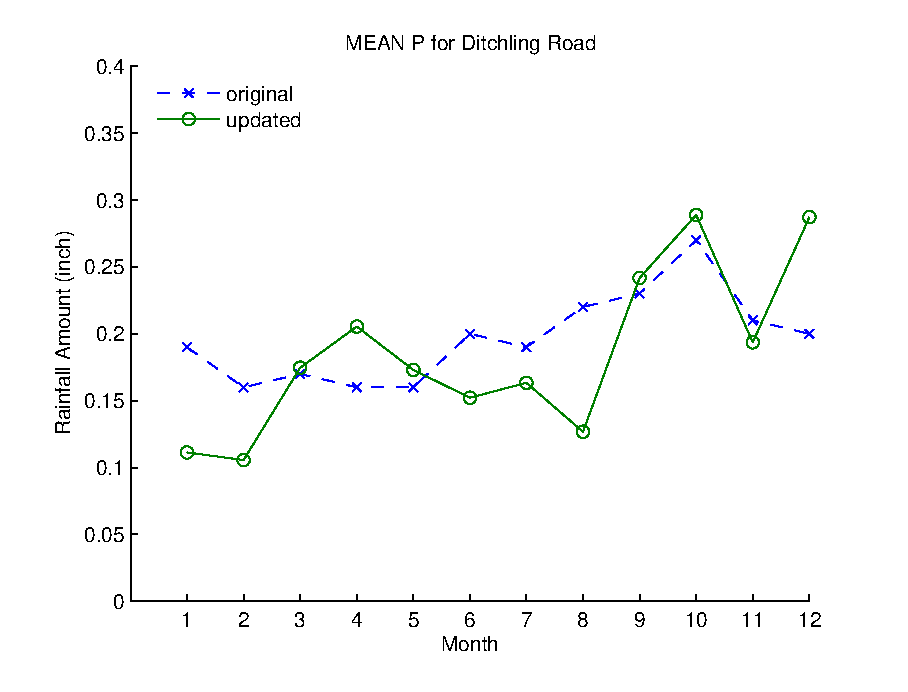
\includegraphics[width=0.49\textwidth]{./img/mean_p_cligen}}
    \subfloat[MX .5P]{\label{fig:mx5p_cligen}
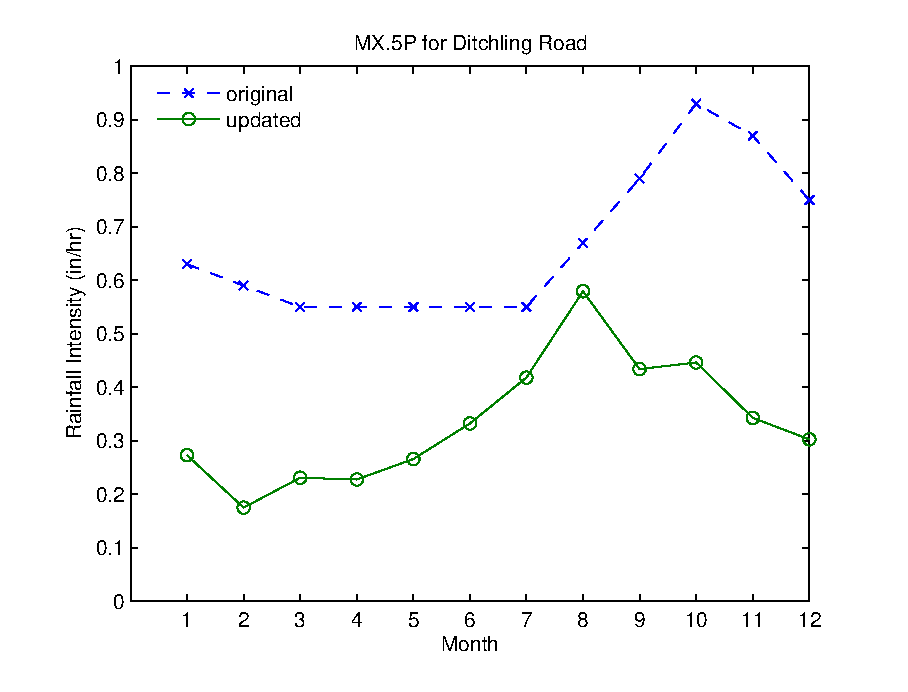
\includegraphics[width=0.49\textwidth]{./img/mx5p_cligen}}
  \caption[Mean daily precipitation depth and mean maximum daily 30-minute
rainfall intensity for each month]{Mean daily precipitation depth (inch) and
mean maximum daily 30-minute rainfall intensity (in/hr) for each month. Note
that the units are in inches, not in millimetres, as CLIGEN requires these
values in inches.}
  \label{fig:mean_p_mx5p_cligen}
\end{figure}

Old CLIGEN (v4.1) did not show much changes in rainfall intensity even though
the rainfall intensity parameter ({MX.5P}) were updated to the lower values when
the input file was prepared. This insensitivity of old CLIGEN (v4.1) is clearly
the result of the unit conversion error previously found by \citet{yu2000-301}.
Correcting the errors in the previous version of CLIGEN resulted in the
decreased rainfall intensity (Figure
\ref{fig:cligen_dr_monthly_max_int_by_month}).

One interesting finding is that when original CLIGEN input file was used for
both climate simulations with old and new CLIGEN, rainfall durations generated
by two CLIGENs were not significantly different so thus resulting intensities.
This finding may be explained by the differences in two versions of CLIGEN. New
CLIGEN (v5.2), as shown earlier, is much more sensitive to changes in rainfall
intensity than old CLIGEN (v4.1), so that, with the CLIGEN input file that has
low rainfall intensity (i.e.\ Updated CLIGEN input), new CLIGEN (v5.2) will
simulate rainfall data with much lower rainfall intensity, hence longer rainfall
durations. This has been shown previously. What is more interesting is that,
in contrast, with CLIGEN input file that has high rainfall intensity
(i.e.\ Original CLIGEN input), new CLIGEN (v5.2) still simulate climate data
with corresponding rainfall intensity, that is high rainfall intensity, hence
short rainfall durations. This is more evident as new CLIGEN (v5.2) generated
shorter annual rainfall durations with original input file (Figure
\ref{fig:cligen_annual_duration}) than old CLIGEN (v4.1) with original (or
updated) input file. However, when mean monthly maxima of daily peak intensity
were compared as shown in Figure \ref{fig:cligen_dr_monthly_max_int_by_month},
new CLIGEN (v5.2) generated lower values for mean monthly maxima of daily peak
intensity than old CLIGEN with both input files. Overall, this finding means
that the improvement of CLIGEN has smaller impacts on weather generations for
regions where high intensity rainfall events are dominant.

Moreover, new CLIGEN with the updated input file simulated a peak monthly
intensity in August (Figure \ref{fig:cligen_dr_monthly_max_int_by_month}) that
can also be seen in the input file (Figure \ref{fig:mx5p_cligen}). This means
that new CLIGEN generates monthly rainfall intensity that are similar
to {MX.5P} values which are calculated from observed weather data. Old CLIGEN,
on the other hand, generated the similar monthly rainfall intensity for both
CLIGEN input files. This implies that old CLIGEN does not recognize the
intensity differences introduced by the different {MX.5P} parameters in the
input files.

Therefore, it is strongly suggested to use new CLIGEN (v5.2) for all future
studies. It is also advisable to review previous CLIGEN input files when
possible.

\subsection{Impact on Subsequent WEPP Simulation}

Runoff and soil erosion rates estimated by WEPP showed the similar responses as
those from the analysis of rainfall generations. This implies that WEPP is
sensitive to the changes of climate data which have been used for the
simulation.

The two identical climate datasets generated by old CLIGEN (v4.1) with two input
files (original and updated) did not affect WEPP estimated annual runoff
(Figures \ref{fig:cligen_annual_runoff_serise_a} and
\ref{fig:cligen_annual_runoff_serise_b}) and soil erosion rates (Figures
\ref{fig:cligen_annual_sloss_series_a} and
\ref{fig:cligen_annual_sloss_series_b}).
There were slight differences between two settings in terms of average annual
runoff and soil loss rates (Table
\ref{tab:SimualtedAnnualRunoffAndSoilLossWithDifferentConfiguration}). The
differences were however unrealistic as average annual soil loss rate was
increased even though average annual runoff was decreased. This suggests that
WEPP may have some issues in estimating runoff and soil loss rates.

The use of two climate datasets generated by new CLIGEN (v5.2) with original and
updated input files resulted in significantly different runoff and soil loss
rates. WEPP simulated considerably lower annual runoff and soil loss rates when
climate data generated by new CLIGEN (v5.2) with updated input file were used
than when climate data generated by new CLIGEN (v5.2) with original input file
were used. This is because of the increased rainfall duration which have
been caused by the decreases in rainfall intensity (Figure
\ref{fig:cligen_annual_duration}). Considering that simulated rainfall amounts
were not much different in both input files of CLIGEN, it is evident that low
rainfall intensity is the reason for the low annual runoff and annual soil loss
rates estimated by WEPP.

Therefore, the implication of the improvement in CLIGEN is relatively small when
CLIGEN was used to simulate climate data for a place where rainfall events
with high intensity are dominant. On the other hand, when CLIGEN was used
to generate climate data for a place where rainfall events with low intensity
are dominant (e.g.\ South Downs, UK), differences of climate data simulated by
old and new CLIGEN would be so great that subsequent WEPP estimations will be
greatly affected and erroneous estimations are inevitable.

In the next section, some examples of previously published studies that may have
been affected by these CLIGEN improvements are subjectively selected and
discussed to highlight the implication of the CLIGEN improvement.

\subsection{Implication for Previously Published Studies with Old CLIGEN}

Published papers that used old CLIGEN, prior to \citet{yu2000-301}, to generate
weather data are theoretically affected by the improvement. The magnitude
of effects can vary depending on characteristics of typical rainfall storms in
study area as shown in the present research.

\paragraph{\citet{baffaut1996-447}} used old CLIGEN to generate 200 years of
climate data for WEPP simulations in order to investigate impacts of CLIGEN
parameters on WEPP-predicted average annual soil loss. The study found that only
five parameters, that are mean precipitation per event, standard deviation of
the precipitation per event, skewness of the precipitation per event,
probability of a wet day following a wet day and probability of a wet day
following a dry day, influenced the estimated average annual soil loss. However,
they found that half hour largest intensity (i.e. {MX.5P}) and the statistical
distribution of the time to peak had less influence on the output. Insensitivity
to {MX.5P} parameter, which \citet{baffaut1996-447} found, could be the result
of the error found in old CLIGEN as \citet{yu2000-301} pointed out.

However, it is also possible that the insensitivity to {MX.5P} was from
the characteristic of rainfall storms in the study area. \citet{baffaut1996-447}
considered Indiana, Alabama, Kansas, Colorado, Washington and Virginia, USA. It
is suggested that storms with high rainfall intensity is common in the central
and eastern United States \citep{ashley2003-3003}. This means that the magnitude
of effects from CLIGEN improvements could be smaller because the studied
area are mostly in the central or eastern US except Washington. As shown in
Table \ref{tab:SimualtedAnnualRunoffAndSoilLossWithDifferentConfiguration},
areas with high rainfall intensity are less influenced by the improvement of
CLIGEN.

Therefore, the information and analysis from \citet{baffaut1996-447} do not
provide any conclusive evidence to determine the effect of improved CLIGEN.

\paragraph{\citet{zhang1996-855}} conducted a study to evaluate the overall
performance of
WEPP in predicting runoff and soil loss under cropped conditions. They also used
old CLIGEN to generate the weather parameters in the WEPP climate input files.
Although they used CLIGEN, not all weather parameters were generated by CLIGEN.
Values for amounts of rainfall, rainfall duration, time to peak intensity and
ratio of mean to peak intensity were directly calculated from measured rainfall
data for each storm at all the sites they considered. This means that their
study may not greatly affected by the change of CLIGEN. As this chapter
suggested, rainfall duration and intensity are the most affected parameters in
WEPP climate inputs.

\paragraph{\citet{baffaut1998-756}} also used old CLIGEN to generate synthetic
weather
series to analyse frequency distributions of measured daily soil loss values and
to determine if the WEPP accurately reproduced statistical distributions of the
measured daily erosion series. The sites that they selected for their study
were in the eastern USA. They selected the study sites based on length of
records, the number of events recorded, and the uniformity of the management
practices. This means that the series of weather data generated by old CLIGEN
may not have been different statistically compared to measured values because
of the high rainfall intensity for their study sites \citep{ashley2003-3003}.
The paper did not include the result of weather simulations. However, it
was indicated that CLIGEN generated data were not statistically different from
monitored weather data. Thus, this paper also elaborates that the implication of
the change of CLIGEN is small when old CLIGEN was used to generated weather
data for areas with high rainfall intensity.

\paragraph{\citet{favis-mortlock1999-329}} conducted a case study from Brazil to
suggest an
approach to quantifying the change in risk of serious erosion for venerable
areas. \citet{favis-mortlock1999-329} used old CLIGEN to generate 100 years of
weather data based on current-climate and, then, used three GCMs to perturb 100
years of CLIGEN generated daily weather data. The area which
\citet{favis-mortlock1999-329} studied has several monsoon characteristics in
addition to the distinct wet and dry seasons \citep{gan2004-47}. This means
that the area have a large variability in rainfall intensity, which implies
that impacts of the change of CLIGEN could be small on the overall result of the
paper. However, it could still be possible that rainfall duration and number of
extreme events could have been overestimated slightly.

The previously published paper that were discussed here used old CLIGEN for
generating weather data. This implies that articles may have been affected by
the previous errors of CLIGEN to a certain extend. However, the information
included in these articles does not have enough details to determine the extend
and the effect of improvements of CLIGEN. Yet, the magnitude of impacts varies
depending on how CLIGEN was used and where CLIGEN was used for. In summary,
it is evident that previously published papers that uses old CLIGEN to
generate weather data for the area, like the central and eastern US or central
South America, where high intensity storm is common are not greatly affected,
at least, not as much as other places like the southern England where low
intensity rainfall is common.

\section{Conclusion}
\label{sec:ImprovedCLIGENConclusion}
The improvement of CLIGEN have important implications on generating synthetic
climate data and subsequent WEPP simulations of runoff and soil loss rates. Old
CLIGEN is not sensitive to changes of rainfall intensity. The previous version
generates the similar climate series with original and updated CLIGEN input
files that have high and low intensity parameters, respectively. However, new
CLIGEN is now sensitive to changes of rainfall intensity which is parameterized
as {MX.5P}. The effect of the improvement of CLIGEN is more (less) significant
for the regions where low (high) intensity rainfall events are dominant.
All previous articles that used old version of CLIGEN may have been affected by
the errors of old CLIGEN to a certain extend. However, the magnitude of impacts
varies depending on how CLIGEN was used and where CLIGEN was used for. It could
have been catastrophic to find out the errors of CLIGEN at the later stage of
this research because the site where this research is based on is South Downs,
UK where impacts of the improvement of CLIGEN are great.

%\nolinenumbers

